\chapter{Resultados}
En este capitulo se presentan los resultados experimentales de el esquema presentado, 


\section{Entorno Experimental}



\subsection{robot}
La plataforma que estamos usando es un robot cartesiano de 3 DOF visto en  \cref{fig:dsc9825}, se utiliza un generador de señal para el voltaje de entrada a los motores de corriente continua, estamos utilizando MATLAB como la interfaz entre el sistema de visión, el control y el generador de funciones.

\begin{figure}
	\centering
	\includegraphics[width=0.5\linewidth]{visio/visio3/coordenadasrobcam2}
	\caption{Representación de un Robot Cartesiano}
	\label{fig:coordenadasrobcam}
\end{figure}


\begin{figure}
	\centering
	\includegraphics[width=0.5\linewidth]{Imagenes/DSC_9825}
	\caption{}
	\label{fig:dsc9825}
\end{figure}



\subsection{\textit{Gripper}}
El \textit{Gripper} que vamos a utilizar es el modelo SCHUNK WSG-50 que aparece en \cref{fig:dsc9821}, tiene un observador de fuerza, utiliza una fuente de 24V, la abertura es de 10 cm y se puede utilizar con MATLAB para ser operado. \\
Para ser usado se necesitó establecer la comunicación con \textbf{MATLAB}, esta es comunicación básica, en la que se manda un paquete de datos que contiene el comando y las opciones, en el apéndice \ref{codewsg50}, aparece el código que se uso.

\begin{figure}
	\centering
	\includegraphics[width=0.7\linewidth]{Imagenes/DSC_9821}
	\caption{\textit{Gripper} modelo SCHUNK WSG-50}
	\label{fig:dsc9821}
\end{figure}

\subsubsection{base del \textit{Gripper}}
Se diseño la base para el \textit{Gripper}, y los dedos, se intenta usar el sensor de fuerza y momento, por lo que uno de los 2 dedos tiene una cavidad para este. en el apéndice \ref{label}, se puede encontrar el diseño que se uso.

en la imagen \ref{label}, se encuentra el resultado




\subsection{cámara}

El sistema de visión usa una cámara RGBD que se muestra en la figura \ref{fig:dsc9822}, se uso un programa entre MATLAB y \textit{Openni} \cite{matlabwrapper}.

La cámara que se uso es el ASUS XTION PRO, su sensor de profundidad tiene un rango operativo de 0,8 metros a 3,5 metros, la resolución de la imagen de color y la imagen de profundidad es $480 \times640$, y la velocidad de fotogramas es 20 cuadros por segundo, ya que es la velocidad de fotogramas del sensor de profundidad. \\




\begin{figure}
	\centering
	\includegraphics[width=0.7\linewidth]{Imagenes/DSC_9823}
	\caption{Camara Asus Xtion live pro}
	\label{fig:dsc9823}
\end{figure}
\begin{figure}
	\centering
	\includegraphics[width=0.7\linewidth]{Imagenes/DSC_9824}
	\caption{}
	\label{fig:dsc9824}
\end{figure}


\section{Protocolo de Experimentación}
%cual es el protocolo? como se disenaron los experimentos?

Los experimentos se diseñaron 

\section{Resultados Experimentales}
A continiacion se presentan los resultados,

En  \cref{labellist} se muestran los resultados











\begin{figure}
	\centering
	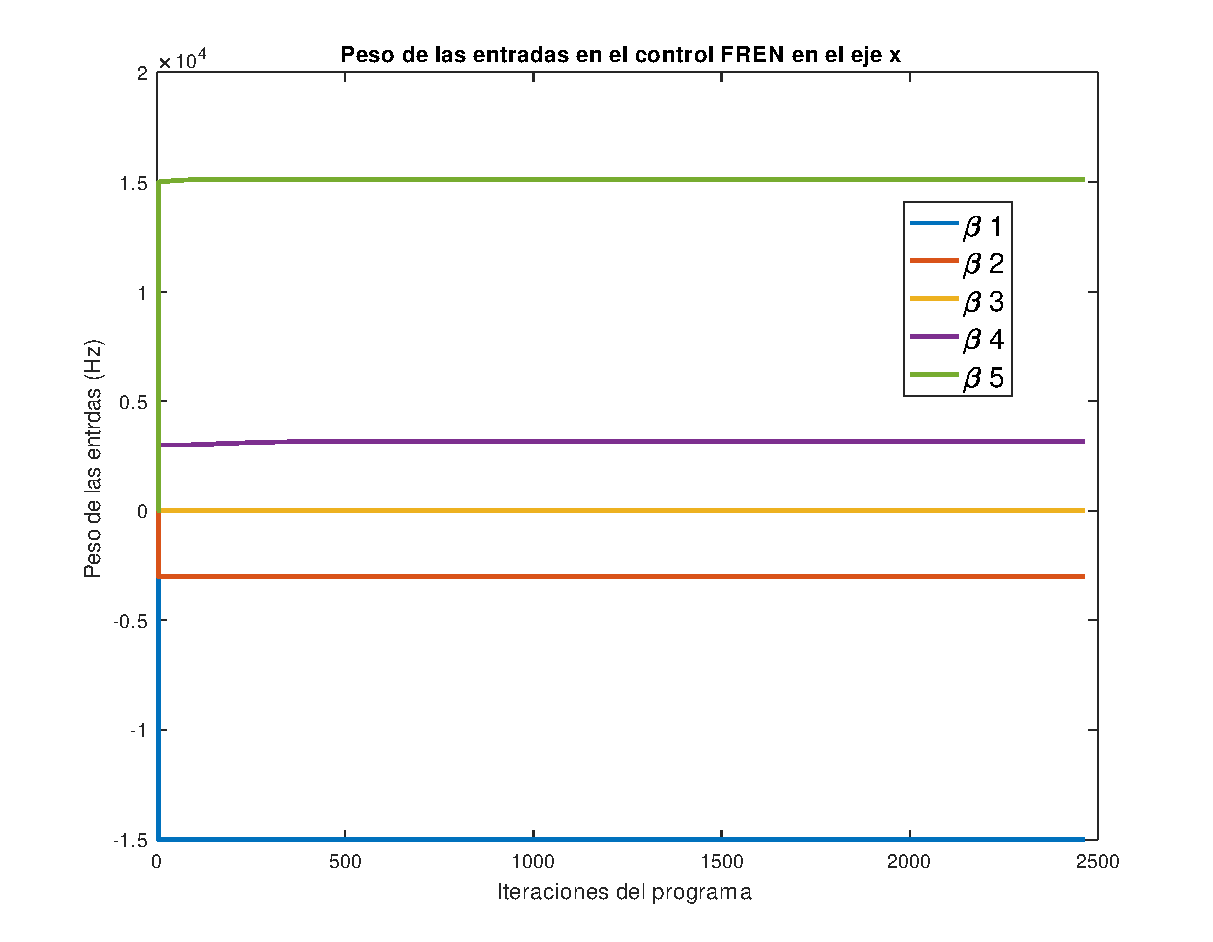
\includegraphics[width=1\linewidth]{visio/graficasderesultados/betasx1}
	\caption{}
	\label{fig:betasx1}
\end{figure}
\begin{figure}
	\centering
	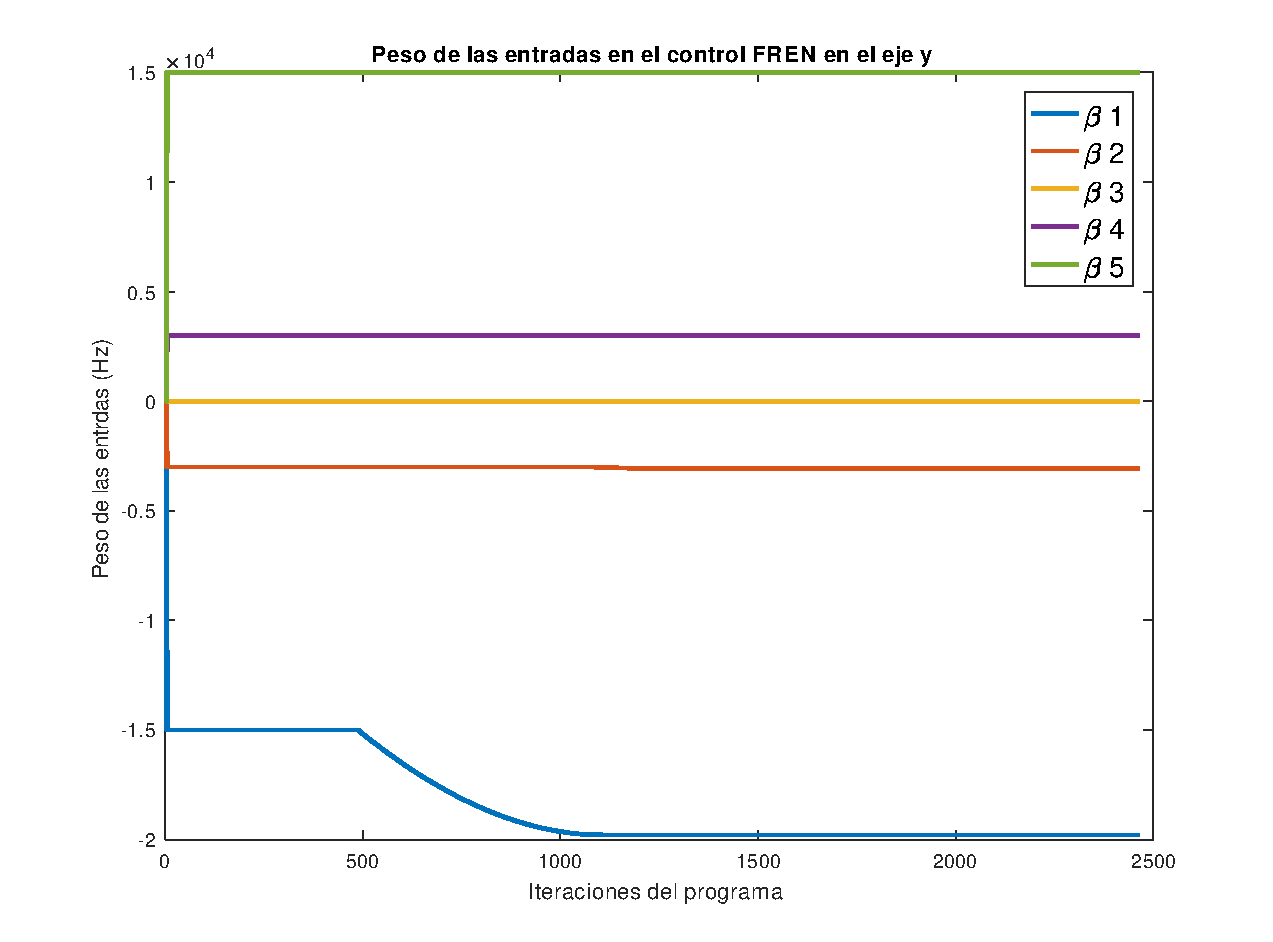
\includegraphics[width=1\linewidth]{visio/graficasderesultados/betasy1}
	\caption{}
	\label{fig:betasy1}
\end{figure}
\begin{figure}
	\centering
	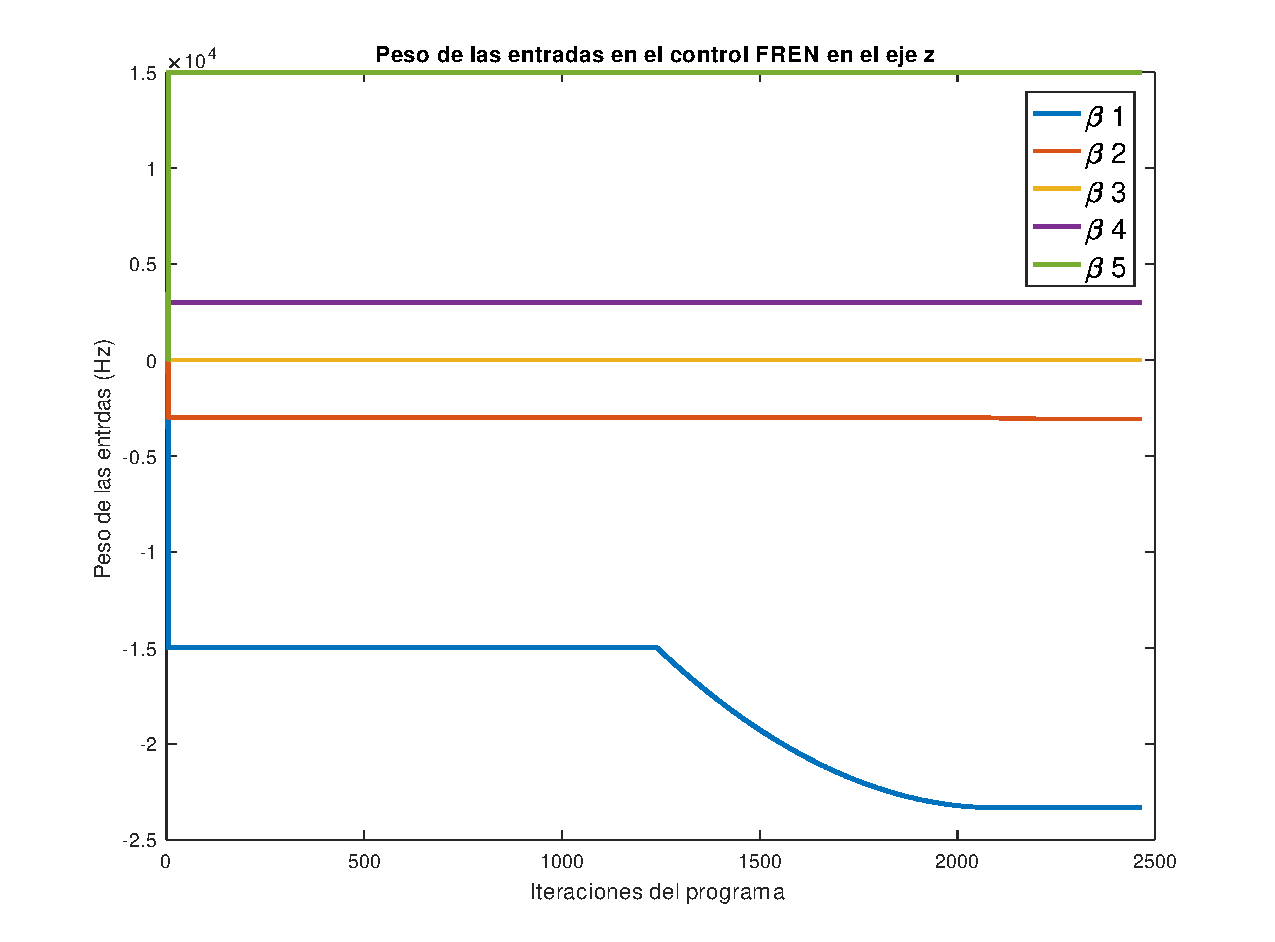
\includegraphics[width=1\linewidth]{visio/graficasderesultados/betasz1}
	\caption{}
	\label{fig:betasz1}
\end{figure}
\begin{figure}
	\centering
	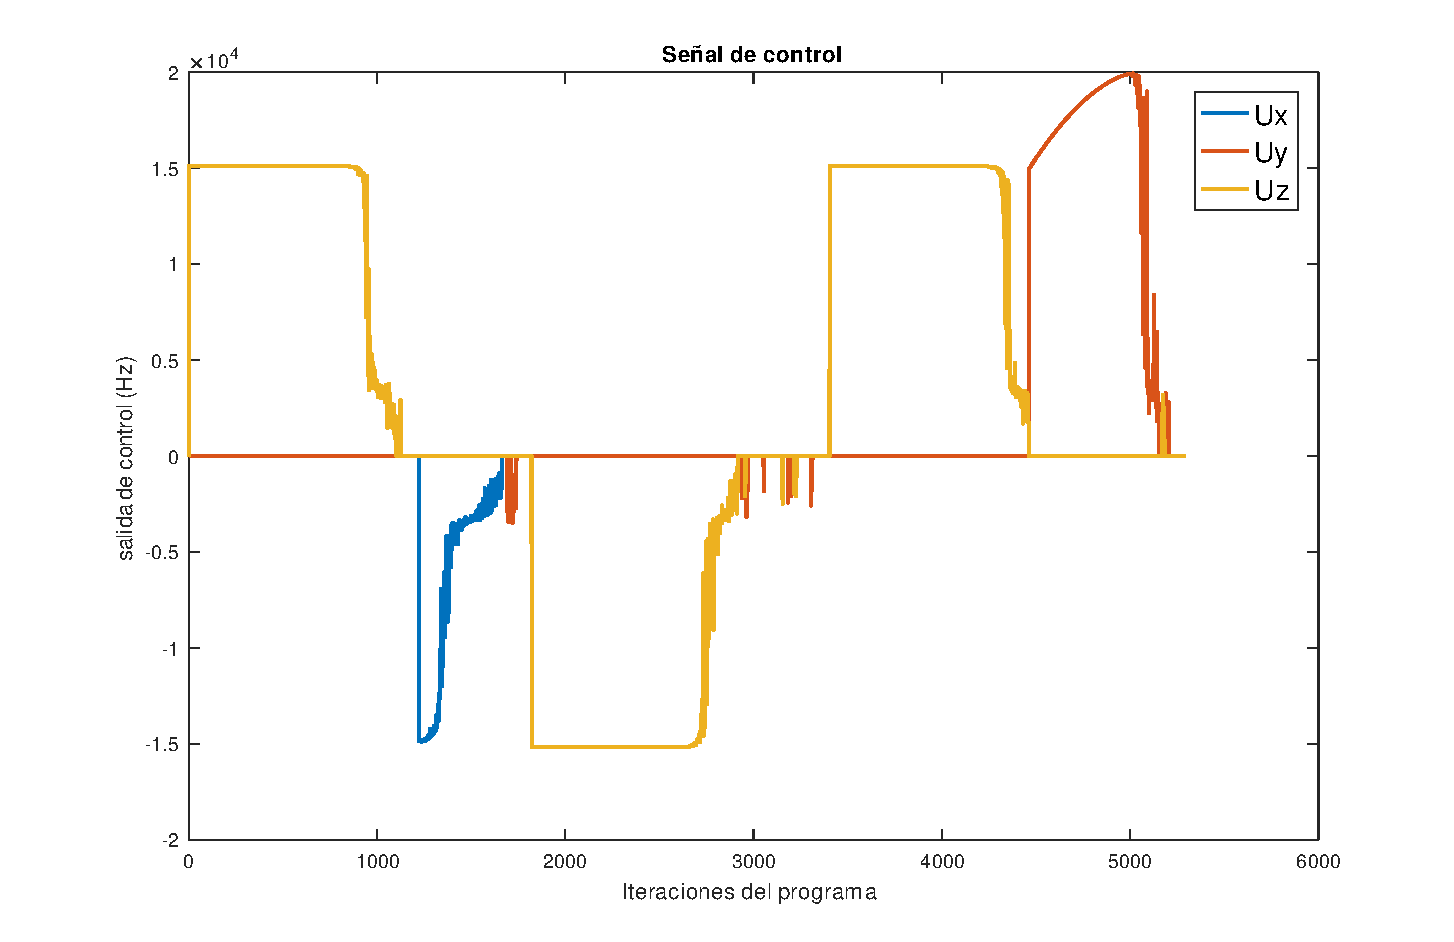
\includegraphics[width=1\linewidth]{visio/graficasderesultados/control1}
	\caption{}
	\label{fig:control1}
\end{figure}
\begin{figure}
	\centering
	\includegraphics[width=1\linewidth]{visio/graficasderesultados/dix1}
	\caption{}
	\label{fig:dix1}
\end{figure}
\begin{figure}
	\centering
	\includegraphics[width=1\linewidth]{visio/graficasderesultados/diy1}
	\caption{}
	\label{fig:diy1}
\end{figure}
\begin{figure}
	\centering
	\includegraphics[width=1\linewidth]{visio/graficasderesultados/diz1}
	\caption{}
	\label{fig:diz1}
\end{figure}
\begin{figure}
	\centering
	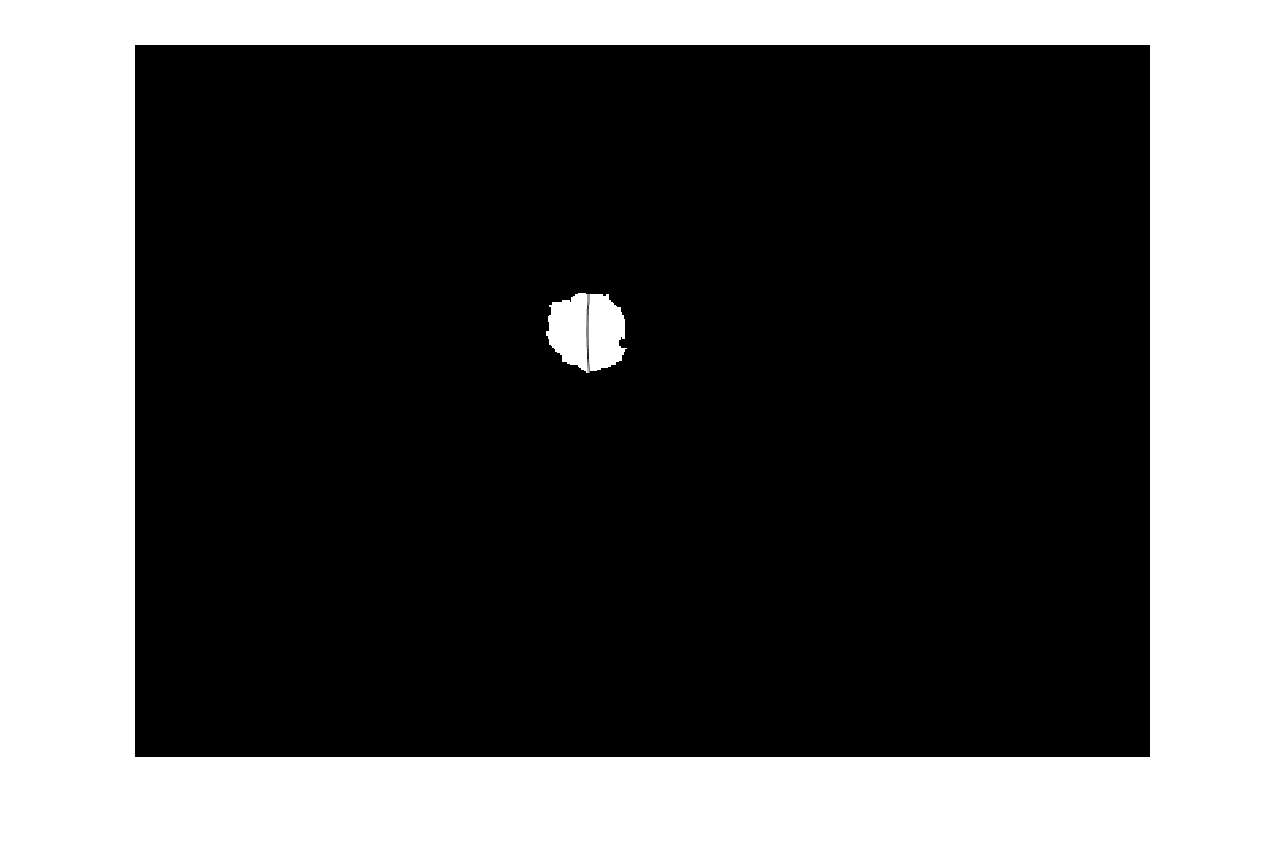
\includegraphics[width=1\linewidth]{visio/graficasderesultados/erz1}
	\caption{}
	\label{fig:erz1}
\end{figure}
\begin{figure}
	\centering
	
\includegraphics[width=1\linewidth]{visio/graficasderesultados/imagen1}
	\caption{}
	\label{fig:imagen1}
\end{figure}
\begin{figure}
	\centering
	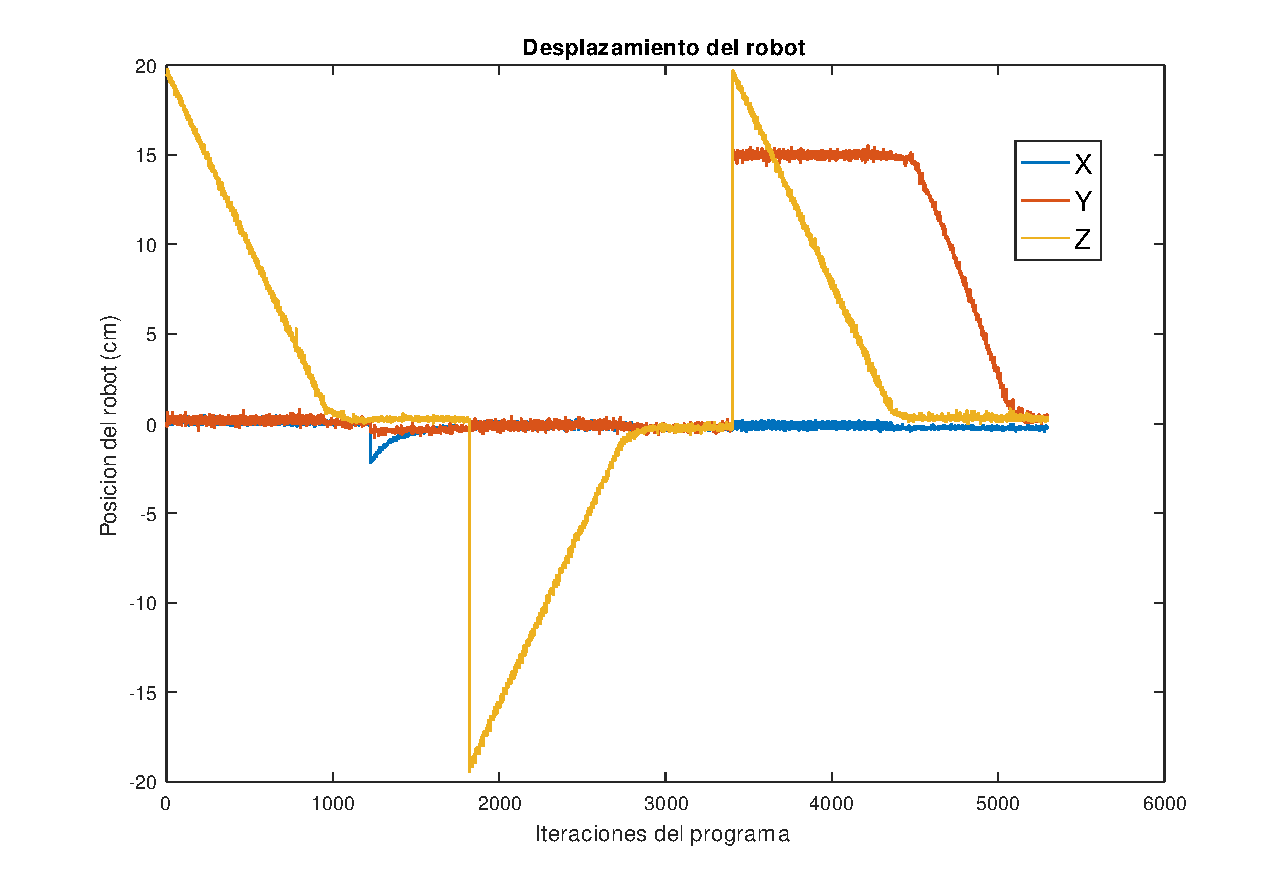
\includegraphics[width=1\linewidth]{visio/graficasderesultados/posicion1}
	\caption{}
	\label{fig:posicion1}
\end{figure}
\begin{figure}
	\centering
	\includegraphics[width=1\linewidth]{visio/graficasderesultados/temp1}
	\caption{}
	\label{fig:temp1}
\end{figure}
\begin{figure}
	\centering
	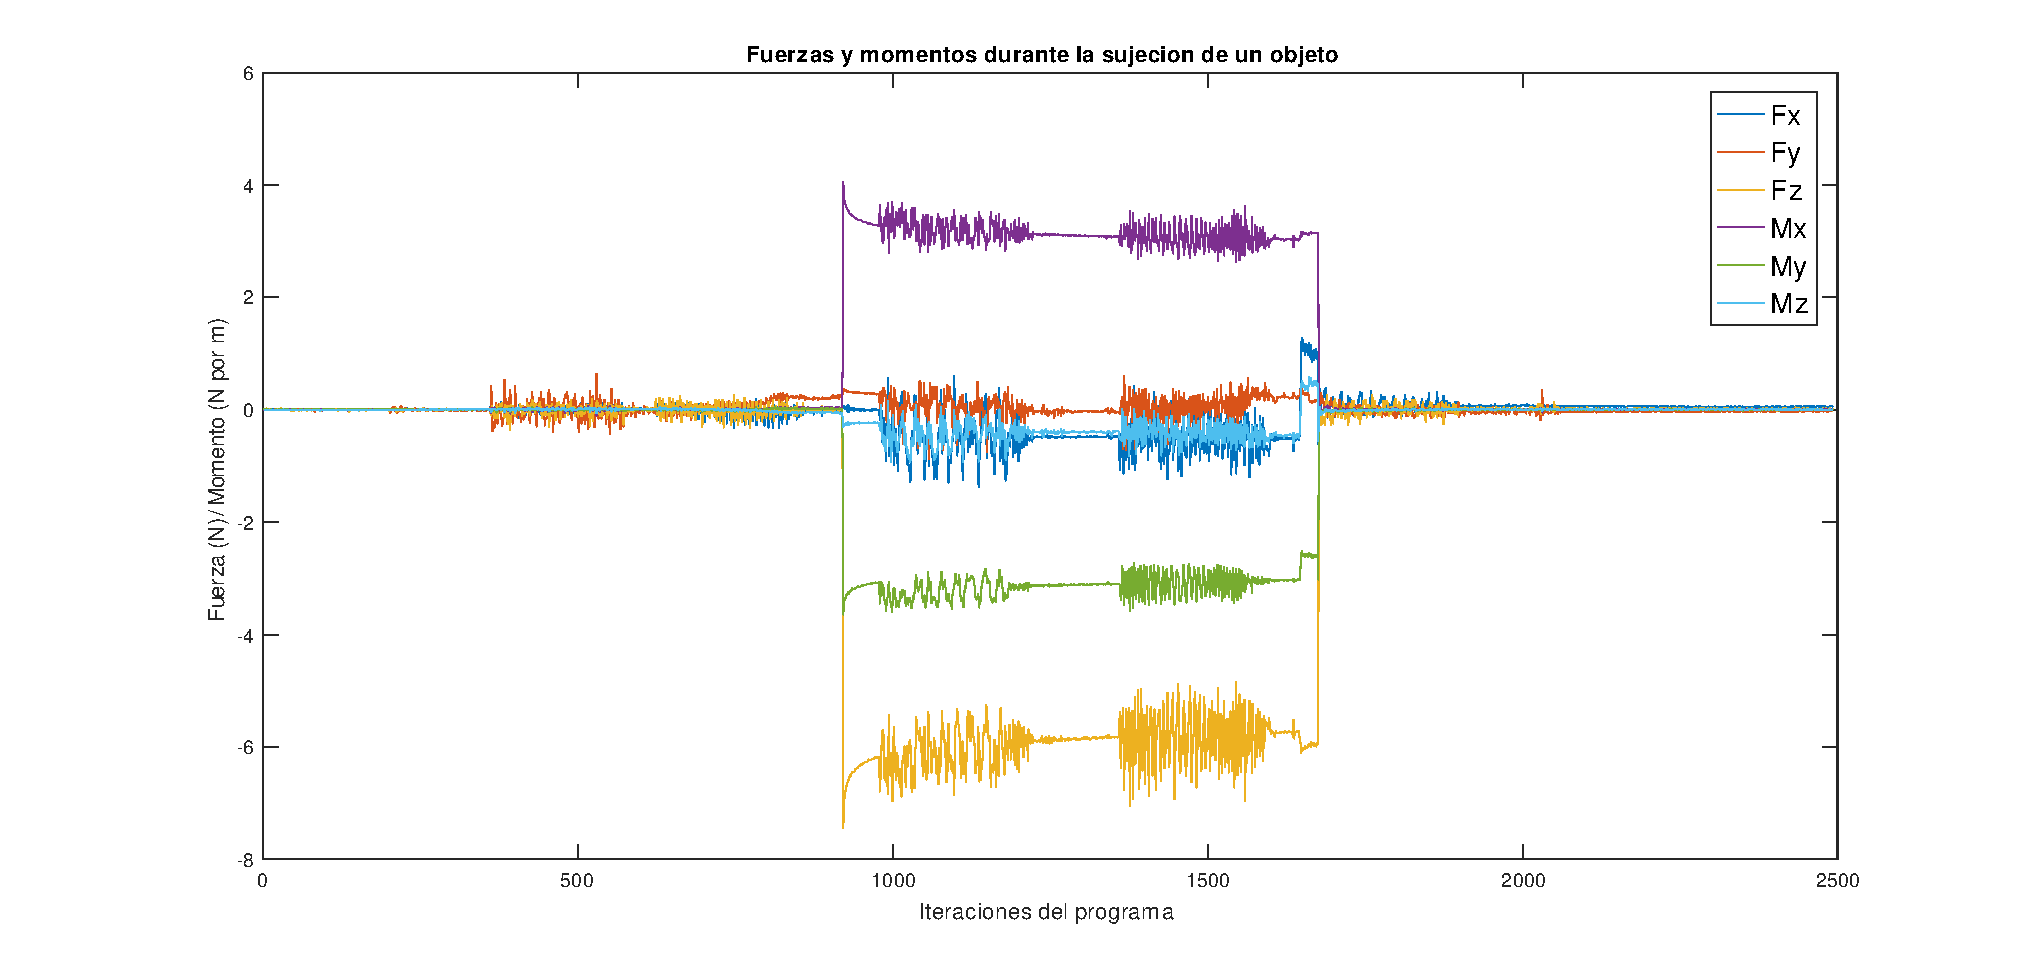
\includegraphics[width=1\linewidth]{visio/graficasderesultados/twist1}
	\caption{}
	\label{fig:twist1}
\end{figure}


\begin{figure}
	\centering
	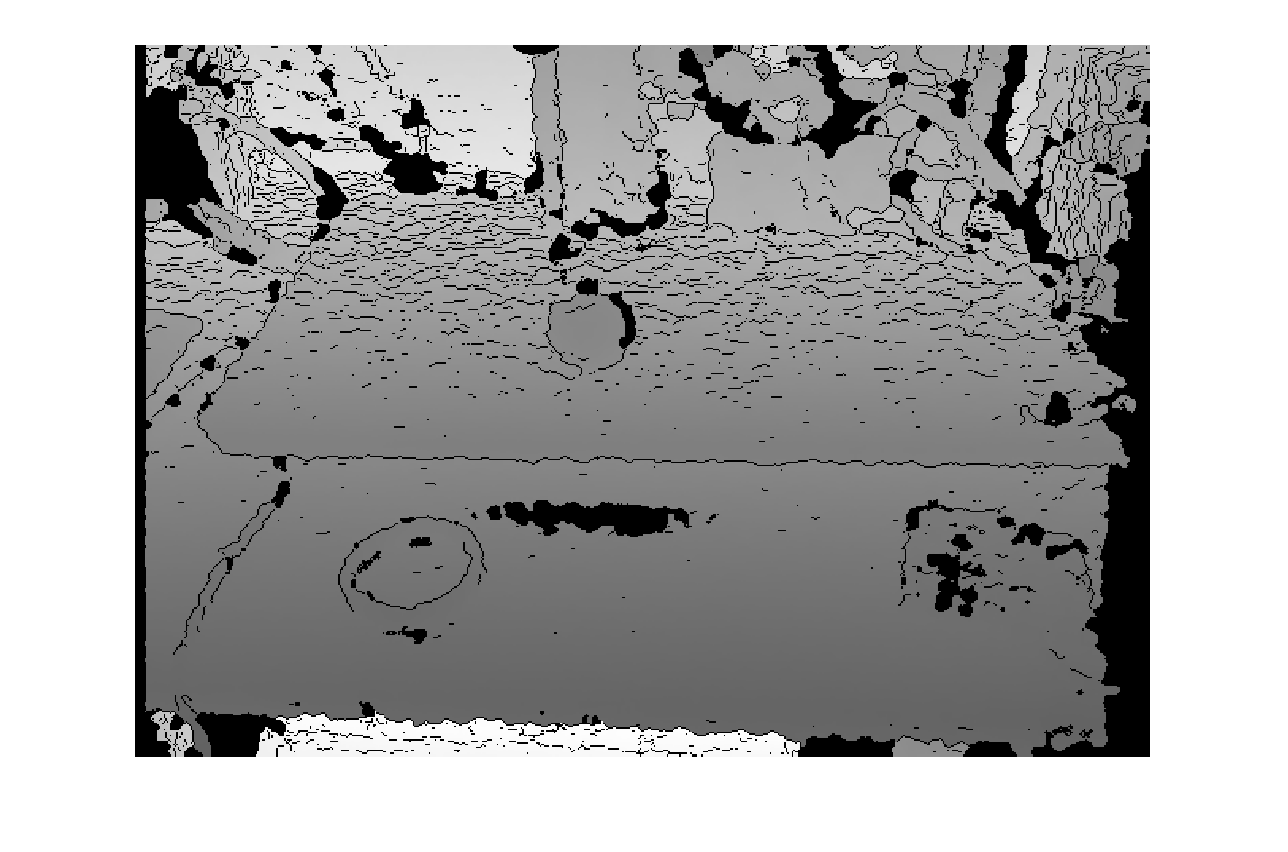
\includegraphics[width=1\linewidth]{visio/graficasderesultados/Dbordes1}
	\caption{}
	\label{fig:dbordes1}
\end{figure}
\begin{figure}
	\centering
	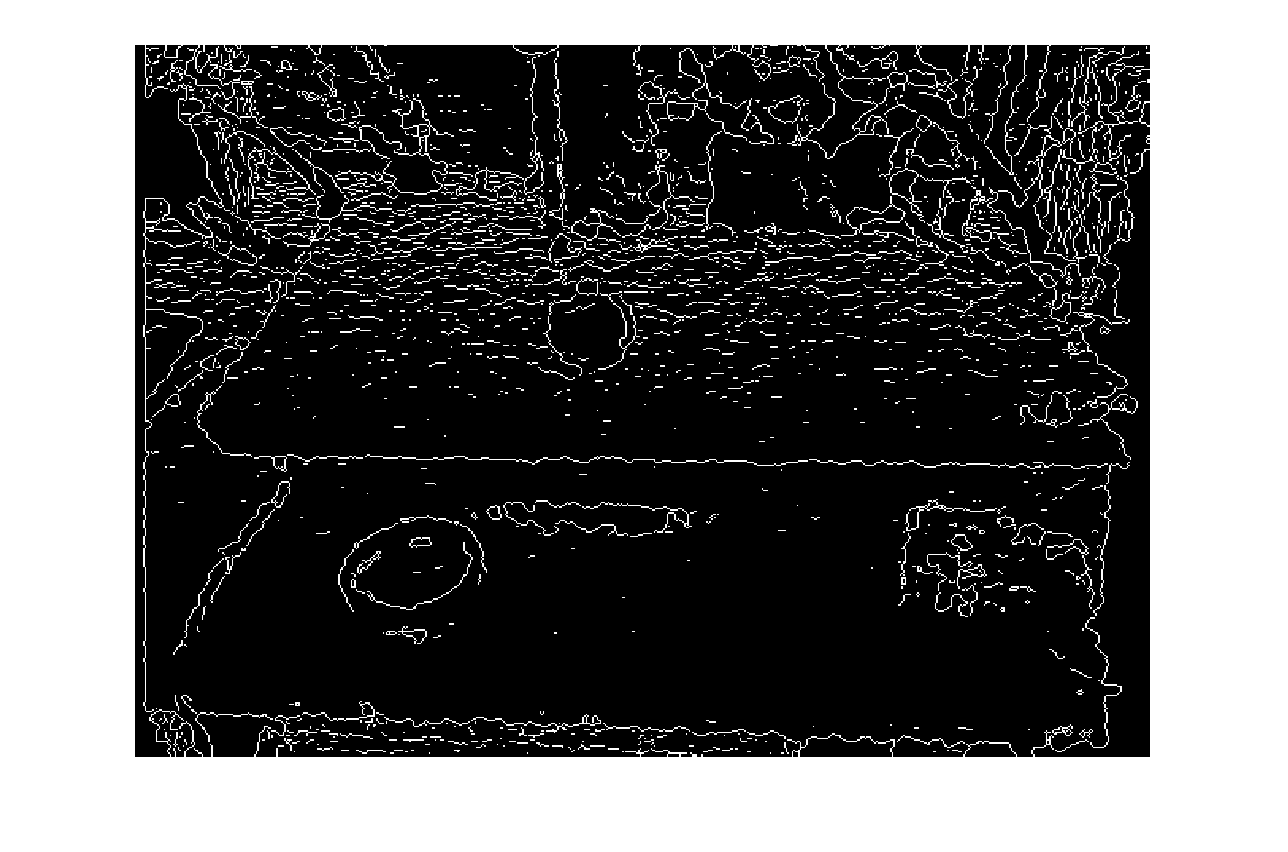
\includegraphics[width=1\linewidth]{visio/graficasderesultados/Dsobel1}
	\caption{}
	\label{fig:dsobel1}
\end{figure}

